We have organized our project into five main tasks as follow:

The first one is the Requirements Elicitation, which is all about we have gathered in this document, namely the analysis and main challenges. the analysis of the existing, and the search for the most relevant features to develop in order to fulfill the needs.

The second one, Project Documentation, is about giving feedback of our progress to the client, the teacher, as well as every person who is interested in our project. This will be continued all over the project duration.

There is a Design and an Implementation task too. Since our project is organized in an iterative mode, it means that we will jump from design to programming as many times as it takes to complete all the tasks.

There will be a test phase, in which we will make sure that all of the features we developed work properly. We will try as much as possible to put them in the iterative cycle as well, so we can go from design, to programming, to test, and so on.

\section{Gantt Chart}
\begin{figure}[!ht]
    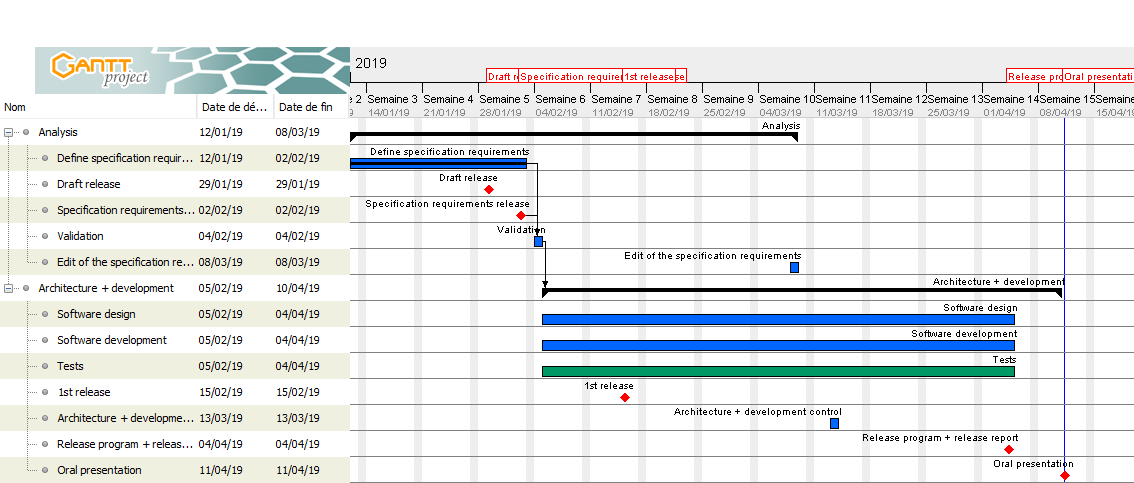
\includegraphics[scale=0.45]{figures/ganttPyTorchfinal.png}
    \caption{Gantt chart}
\end{figure}
\pagebreak
